%%==================================================
%% chapter03.tex for SJTU Master Thesis
%% Encoding: UTF-8
%%==================================================

\chapter{基于过完备字典技术的重构上采样方法}
\label{chap:faq}

本章先介绍本文的应用过完备稀疏字典技术的重构上采样方法的计算框架,引出过完备稀疏字典方法重点研究的两个问题,并指出这两个问题之间的联系。再针对这两个问题,详细介绍本文提出的解决方案。

\section{应用过完备字典技术的重构上采样方法的计算框架}

根据第三章流体重构的上采样框架图~\ref{simulationframework},本章的重构上采样方法要实现的内容是将低精度网格的速度场数据还原到对应的高精度网格上。在图像处理领域,有很多针对图像做重构上采样的方法,其中相对简单并且被广为使用的方法有传统的双三次插值、双线性插值、邻居嵌入算法~\cite{chang2004super}等,这类方法具有简单、易实现的特点,但重构的效果不是很理想。后来,出现了一批基于机器学习的图像超分辨算法,如基于Example的学习~\cite{freeman2002example}~\cite{kim2008example}算法和基于稀疏编码的过完备字典学习算法等。

基于Example的学习算法可以较好地重构出高精度图像的细节,特别是Yang在2013年提出的基于In-Place Example Regression~\cite{yang2013fast}的快速超分辨算法,作者指出该算法不仅有较快的重构速度,而且几乎不会引入人工痕迹和模糊效果。该算法的核心思想是在重构上采样时,先用双三次插值的算法放大低精度图像patch的低频信号,根据低精度图像的低频信号原位找到对应的高精度图像patch所在的位置,再通过一阶回归算法,提取低精度图像的低频信号与高频信号之间的关系和高精度图像的低频信号来预测高精度图像高频信号部分。又因该算法在处理每个patch时,计算的是取重叠像素后的多个patch之间的平均值,故具有较好的平滑性。

基于过完备稀疏训练字典技术的图像超分辨方法假设直接从数据中提取其表示形式可以更好地重构出自然现象的复杂数据结构。该算法以低精度图像为输入,以patch为单位处理图像,获取其稀疏表示形式,然后再与高精度过完备稀疏字典线性组合,达到重构高精度图像的目的。本文利用基于过完备稀疏字典技术可以更好地适应特定的数据这一特点,学习一对能够表示流体低—高精度速度场数据对应关系的过完备稀疏训练字典,并重构上采样低精度速度场到高精度网格中。图~\ref{fig:dictionaryFramework}为本文的重构算法框架图。

\begin{figure}
  \centering
   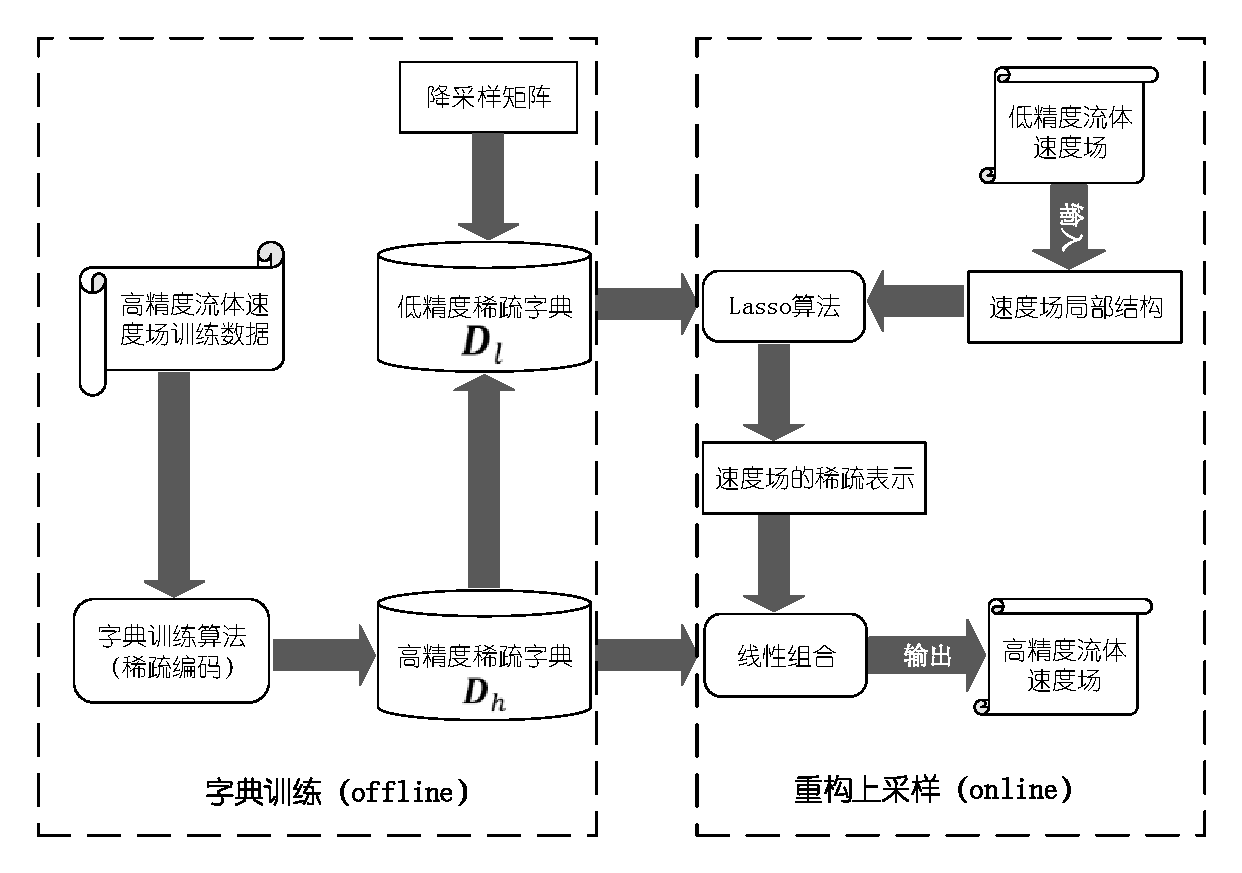
\includegraphics[height=4.1 in]{chap4/dictionaryFramework}
  \bicaption[fig:dictionaryFramework]{}{过完备字典技术的整体框架}{Fig}{The whole framework for over-complete dictionaries}
\end{figure}

从框架图可以看出,该框架主要分为两大部分,即应用过完备稀疏字典技术的重构上采样部分和基于稀疏编码技术的过完备字典的训练部分,其中,过完备字典的训练是一个离线训练的过程,重构上采样方法以低精度网格的速度场数据和离线生成的低精度过完备稀疏字典为输入,使用基于稀疏编码技术的分解算法获得流体速度场的稀疏表示,再线性组合流体的稀疏表示和高精度稀疏字典,即可恢复高精度网格的流体速度场。本章的余下部分将会详细介绍过完备字典的训练过程和过完备字典的重构上采样方法。

\section{过完备字典的训练}
\label{sub:dics}

通常来说,对于一个信号向量\({ \boldsymbol {\tilde f}} \in {\boldsymbol R}^{m \times 1}\),如果我们可以通过线性组合集合\(\boldsymbol d_i \in {\boldsymbol R}^{n \times k},i=1,…,n\)中很少的一些原子,达到尽可能近似地重构出原信号\({\boldsymbol f}  \in {\boldsymbol R}^{n \times 1}\)的目的,我们称这样的一个集合\(\boldsymbol d_i\)为过完备稀疏字典。

学习一对过完备稀疏训练字典,是本文研究的一个重点内容。一对过完备字典可以弥补低-高网格精度的流体速度场数据之间的信息差,在流体速度场数据的重构上采样算法中起到关键性的作用。在图形图像领域,Mairal和Bach~\cite{mairal2009online}~\cite{mairal2010online}等人提出了基于稀疏编码技术的快速在线字典学习方法,并发布了求解各种稀疏近似问题的优化工具箱;Yang等人在图像超分辨领域提出的联合训练字典方法,将高精度图像降采样到低精度空间,再将低-高精度信息放到一个向量中,使用稀疏编码技术~\cite{lee2006efficient}训练生成一对过完备的稀疏字典。本文借鉴Yang的联合训练字典方法重构上采样流体速度场数据,下面的问题描述部分将会详细给出联合双字典技术求解的问题。

\subsection{联合训练字典的问题描述}
\label{chap:problem}

假设有两对特征空间:潜在空间$\boldsymbol X \in \boldsymbol R^{d1} $和观察空间$\boldsymbol Y \in \boldsymbol R^{d2} $,观察空间的信号是稀疏的,即信号可通过某一字典求得其稀疏表示形式。潜在空间的信号是我们希望恢复或者重建的信号。存在映射函数 $F:\boldsymbol X \rightarrow \boldsymbol Y$(不需要是线性的,并且可以是未知的),根据关系$\boldsymbol y = F(\boldsymbol x)$ ,把空间$\boldsymbol X$中的信号$\boldsymbol x$映射到与之一致的空间$\boldsymbol Y$中的信号$\boldsymbol y$。此处,我们假设映射函数是近似内射的,否则不能从$\boldsymbol Y$推断$\boldsymbol X$。

成对空间的信号恢复问题类似于压缩感知问题。在压缩感知的内容中,观察空间和潜在空间由一个线性随机映射函数$F$连接起来。字典$\boldsymbol D_x$通常被选来做数学形式上定义的基(比如小波),$\boldsymbol D_y$则是直接利用线性映射$F$从$\boldsymbol D_x$中获得的。

我们的问题是分别为空间$\boldsymbol X$和$\boldsymbol Y$找一对字典$\boldsymbol D_x$和$\boldsymbol D_y$ ,这样给定任何信号 ,我们都可以用它计算出给定信号关于字典$\boldsymbol D_y$的信号稀疏表示,再线性组合字典$\boldsymbol D_x$恢复与之一致的潜在信号$\boldsymbol x \in \boldsymbol X$ 。在形式上,一对理想字典$\boldsymbol D_x$和$\boldsymbol D_y$,对于任何信号对$\{\boldsymbol y_i, \boldsymbol x_i\}$ ,都应满足下列方程组:
\begin{equation}
\label{eq:decx}
\boldsymbol \alpha_i = \min_{\boldsymbol \alpha_i}||\boldsymbol y_i - \boldsymbol D_y \boldsymbol \alpha||_2^2 + \lambda||\boldsymbol \alpha_i||_1
\end{equation}

\begin{equation}
\label{eq:decy}
\boldsymbol \alpha_i = \min_{\boldsymbol \alpha_i}||\boldsymbol x_i - \boldsymbol D_x \boldsymbol \alpha||_2^2 + \lambda||\boldsymbol \alpha_i||_1
\end{equation}

其中$\{\boldsymbol x_i\}_{i = 1}^N$是$\boldsymbol X$中的训练采样,$\{\boldsymbol y_i\}_{i = 1}^N$是$\boldsymbol Y$中关于$\boldsymbol y_i = F(\boldsymbol x_i)$的训练采样,$\{\boldsymbol \alpha_i\}_{i = 1}^N$是信号的稀疏表示。在一些稳健的情况下,根据方程~\ref{eq:dec}推导的稀疏表示$\boldsymbol \alpha$可以被用来很好地恢复$\boldsymbol x$。然而,在更一般的场景中,即映射函数$F$未知并且可能是非线性时,则不可以应用压缩感知定理。

\subsection{联合训练字典方法}

在图像超分辨领域,Yang提出的联合稀疏字典技术取得了不错的成果,本章节的该部分将会简单介绍该字典训练方法在流体速度场的应用。

给定一组高精速度流体速度场训练数据对$P = \{\boldsymbol u^h,\boldsymbol u^l\}$, 其中,$\boldsymbol u^h$表示高精度网格空间的速度场训练数据,$\boldsymbol u^l$表示相应的使用映射函数$F$计算出的低精度网格空间的流体速度场训练数据。根据问题描述部分~\ref{chap:problem}给出的稀疏训练字典应该满足的关系,我们可以写出流体速度场稀疏字典需要满足的方程组:
\begin{equation}
\label{eq:dec}
\boldsymbol \alpha = \min_{\boldsymbol \alpha}||\boldsymbol u^l - \boldsymbol D_l \boldsymbol \alpha||_2^2 + \lambda||\boldsymbol \alpha||_1
\end{equation}
\begin{equation}
\boldsymbol \alpha = \min_{\boldsymbol \alpha_i}||\boldsymbol u^h - \boldsymbol D_h \boldsymbol \alpha||_2^2 + \lambda||\boldsymbol \alpha||_1
\end{equation}

其中,$\boldsymbol D_l$表示低精度稀疏字典,$\boldsymbol D_h$表示高精度稀疏字典,$\boldsymbol \alpha$表示流体速度场数据的稀疏表示。

如果单独求解两个特征空间的稀疏字典,不能表示低-高精度流体速度场数据之间的对应关系。并且对同一信号的低-高精度训练数据,其稀疏表示形式是相同的。故可以将上述两个方程式合并成如下形式:
\begin{equation}
\min_{\boldsymbol D_h, \boldsymbol D_l, \boldsymbol \alpha}(||\boldsymbol u^h - \boldsymbol D_h \boldsymbol \alpha||_2^2 + ||\boldsymbol u^l - \boldsymbol D_l \boldsymbol \alpha||_2^2) + \lambda||\boldsymbol \alpha||_1
\end{equation}

其中,$\lambda$为拉格朗日算子,主要用来平衡稀疏系数的稀疏性。设 $N$ 和 $M$ 分别为低-高精度流体局部结构数据的维度, 再将上述式子中的两个训练数据集放到一个向量中,重新整理后可将双特征空间的稀疏编码问题表示成如下形式:
\begin{equation}
\label{eq:YangDic}
\min_{\boldsymbol D_h, \boldsymbol D_l, \boldsymbol Z}||\boldsymbol X_c - \boldsymbol D_c \boldsymbol Z||_2^2 + \lambda(\frac{1}{N} + \frac{1}{M})||\boldsymbol Z||_1
\end{equation}

其中,$\boldsymbol X_c = \left[\begin{array}{c} \frac{1}{\sqrt N}\boldsymbol u^h \\
\frac{1}{\sqrt M}\boldsymbol u^l\\
\end{array}
\right]
$,
$\boldsymbol D_c = \left[\begin{array}{c} \frac{1}{\sqrt N}\boldsymbol D_h \\
\frac{1}{\sqrt M}\boldsymbol D_l\\
\end{array}
\right]$,分别是是低-高精度样本数据和稀疏字典的组合形式。

联合训练字典方法巧妙地将低-高精度的流体速度场样本数据放到了一个向量中,这样可以得到一个基本形式与一般的过完备训练字典方法形式相同的方程式~\ref{eq:YangDic},故可用现有的稀疏编码算法学习一对低-高精度空间的稀疏字典$\boldsymbol D_l$和$\boldsymbol D_h$。

稀疏编码算法是一种无监督学习算法,该算法在一组过完备的基向量中寻找样本数据的稀疏表示。给定一个无标签的输入数据,稀疏编码算法可以学习生成一些能捕获输入数据高级别特征的基函数。不同于一般的无监督学习算法,如PCA等,稀疏编码算法可以用来学习过完备基的集合,即学习生成的基的数量要远大于输入信号的维度。在基于稀疏编码的过完备训练字典方法中,这些训练生成的基原子的集合即为过完备稀疏字典。

\subsection{降采样联合字典方法}

根据章节~\ref{chap:problem}问题描述部分指出,信号的稀疏表示不仅在高精度空间是最优的,还要保证在低精度空间是最优的,才能准确低恢复出原信号。而Yang提出的联合学习字典方法将低-高精度空间数据放到一个向量中学习,那么根据稀疏编码技术学习生成的稀疏字典,只能保证求得的稀疏表示形式在低-高精度联合空间内是最优的。但是在重构高精度空间数据时,只有低精度空间的数据向量作为输入,故其求得的稀疏表示也只能保证在低精度空间是最优的。由上述分析可知,Yang提出的联合训练字典学习方法存在训练字典的最优空间和重构上采样的最优空间不一致问题,即我们可以认为根据稀疏字典学习的稀疏表示代表的信号与重构上采样方法分解求得的稀疏表示代表的信号不一致,故从理论上讲,该训练字典方法学习生成的稀疏训练字典不能保证重构上采样结果的准确性。Yang针对其提出的联合训练字典方法存在的重构结果不准确的问题,在2013年的论文~\cite{yang2012bilevel}中提出了改进方案。该方案使用一个通用的双向稀疏编码模型来学习具有一对信号空间的字典,达到提高重构结果准确性的目的,但是该改进模型仍然无法达到流体动画领域所需要的精度。

本文提出的过完备稀疏字典方法,为了保证在稀疏字典学习阶段分解信号的稀疏表示的最优空间与重构上采样阶段分解信号的稀疏表示的最优空间尽量保持一致,对联合训练字典方法的输入向量做了一些改进。在过完备字典的训练学习阶段,我们只收集高精度流体速度场的样本数据,并将其展开放到一个向量中,使用稀疏编码技术学习生成对应的高精度过完备稀疏字典。然后再使用低精度速度场数据与高精度速度场数据之间的映射关系,生成一个适用于低精度速度场的过完备稀疏字典。

首先,给定高精度流体速度场训练数据集$\{\boldsymbol u_i\}_{i = 1}^K$,其中$\boldsymbol u_i \in \boldsymbol R^{n \times 1}$,类似于方程式~\ref{eq:YangDic},本文提出的基于稀疏编码技术的高精度稀疏字典$\boldsymbol D_h$可以用如下式子表示:
\begin{equation}
\label{eq:trainning}
\min_{\boldsymbol D_h,\{\boldsymbol \alpha_i\}_{i = 1}^K} \sum||\boldsymbol u_i - \boldsymbol D_h\boldsymbol \alpha_i||_2^2 + \lambda ||\boldsymbol \alpha_i||_1
\end{equation}

并且,高精度稀疏字典$\boldsymbol D_h$需要满足如下表示的约束条件:
\begin{equation}
\label{eq:condition}
s.t. \ \ \ ||\boldsymbol D_h(:k)||_2 \le 1, \forall k \in \{1, 2, ...,N\}
\end{equation}

其中,$\boldsymbol D_h(:k)$表示高精度稀疏字典$\boldsymbol D_h$的第$k$列。通常,过完备稀疏字典$\boldsymbol D_h$的每一列表示一个原子项或者一个基原子。

此处,我们使用的方程式与联合稀疏字典推导的方程式~\ref{eq:YangDic}具有相同的形式,故也可使用稀疏编码算法~\cite{lee2006efficient}求解。方程式~\ref{eq:trainning}及其约束条件~\ref{eq:condition}需要求解两个未知量,即稀疏字典$\boldsymbol D_h$和稀疏表示系数$\{\boldsymbol \alpha_i\}_{i = 1}^K$,我们无法在一个方程式中同时求解两个未知量。但是,我们可以分别固定变量$\boldsymbol D_h$和$\{\boldsymbol \alpha_i\}_{i = 1}^K$,即假设其中一个变量已知,再来求解另一个未知量,然后通过迭代的方法直到最终的结果都收敛。当过完备字典$\boldsymbol D_h$为已知量时,可以用统计学领域广泛使用的Lasso算法求解稀疏表示系数$\{\boldsymbol \alpha_i\}_{i = 1}^K$,当稀疏表示系数$\{\boldsymbol \alpha_i\}_{i = 1}^K$为已知量时,可以把求解过完备字典$\boldsymbol D_h$的问题当作一个标准的Quadratically Constrained
Quadratic Programming(QCQP)问题。

\begin{figure}[ht]
  \centering
  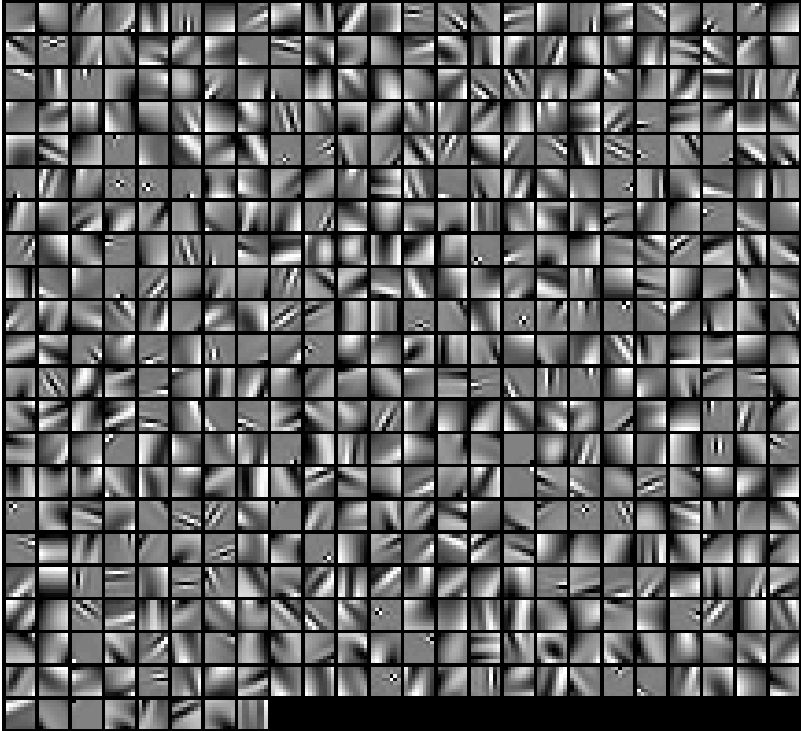
\includegraphics[width=0.49\textwidth]{chap4/regx}
  \hspace{0.1cm}
  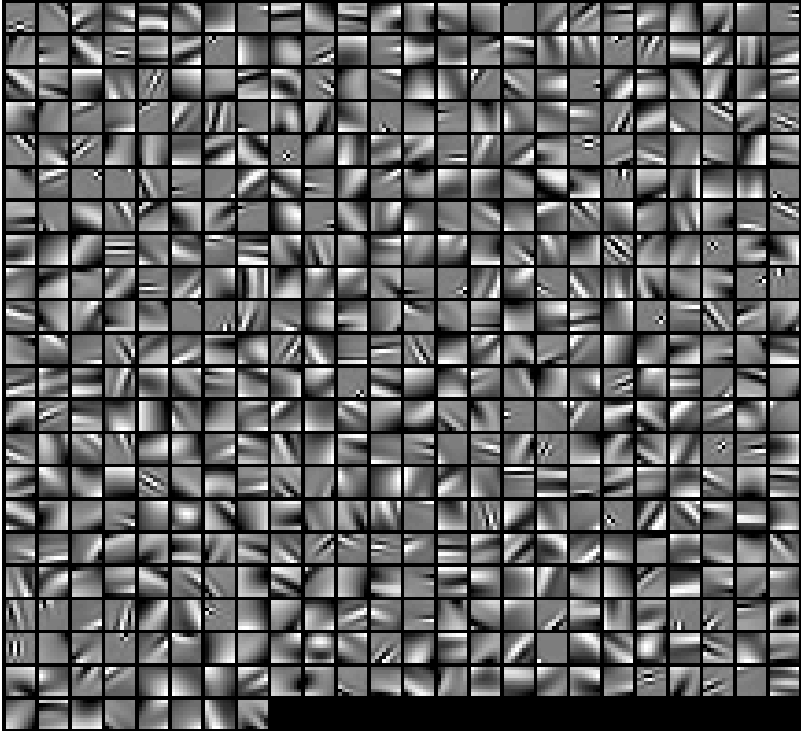
\includegraphics[width=0.49\textwidth]{chap4/regy}
   \newline \ \ \ \ \ \ \ \ \ \ \ \ \ \ \ \ \ \ \ \ \ (a) \ \ \ \ \ \ \ \ \ \ \ \ \ \ \ \ \ \ \ \ \ \ \ \ \ \ \ \ \ \ \ \ \ \ \ \ \ \ \ \ \ \ \ \ \ \ \ \ \ \ \ \ \ \ \ \ \ \ \ \ \ \ \ \ \ \  (b)\ \ \ \ \ \ \ \ \ \ \ \ \ \ \ \ 
  \bicaption[fig:dictionaries]{过完备稀疏字典的可视化效果图}{训练生成的过完备稀疏字典的原子项的可视化示意图。(a)水平方向速度场的稀疏字典。(b)垂直方向速度场的稀疏字典}{Fig}{Visualization of velocity field atoms captured from overcomplete dictionaries trained by equation~\ref{eq:trainning}. (a) the dictionary for the vertical velocity field. (b) the dictionary for the horizontal velocity field.}
\end{figure}

图~\ref{fig:dictionaries}展示了根据上述方程式训练生成的稀疏字典的原子项的可视化示意图。其中,图(a)展示的是用水平方向速度场数据生成的稀疏字典,图(b)展示的是用垂直方向速度场数据生成的稀疏字典。在训练图中所示稀疏字典时,使用的代表流体局部细微结构的patch的大小为$8 \times 8$。仔细观看示意图,可以发现其展示的稀疏字典的原子项有22行、24列,故可视化效果图的底部有$16(24 \times 22 - 512 )$个原子项是全黑的,即那些原子项是不存在的。仔细观察可视效果图中的有效原子项,可以看出流体速度场的字典原子捕获到的高精度边缘展示了不同的流体速度场梯度。

根据第三章的给出的本文流体动画重构上采样基本框架图可以看出,该框架中的低精度速度场数据和高精度速度场数据之间的映射关系可以通过降采样步骤中使用的降采样矩阵表示。要计算出一个适用于低精度流体速度场的过完备稀疏字典,可以通过线性组合降采样矩阵和高精度稀疏字典获得,故低精度稀疏字典的求解过程可以表示成如下形式:
\begin{equation}
\boldsymbol D_l= \boldsymbol {SD}_h
\end{equation}

其中,$\boldsymbol S$ 表示一个大小为$m \times n, m < n $的降采样矩阵,$m$和$n$分别表示低精度和高精度速度场数据的维度。

相较于把低精度空间和高精度空间的流体速度场数据放到一个向量中训练的方法,本文提出的训练字典方法避开了信号的稀疏表示在学习稀疏字典时的最优空间和重构上采样时的最优空间不一致问题,并且本文第五章的实验部分证明,使用该方法生成的低精度稀疏字典更适用于流体的低精度速度场数据。
 
 为了更好地表示流体速度场的局部细微结构,在下面章节的重构上采样算法部分,提取输入的低精度流体速度场数据的高频部分之后再执行重构上采样步骤。为了与重构上采样的输入数据保持一致,该章节的流体速度场训练样本数据也是在执行提取高频部分的预处理操作之后,在对提取出的高频部分进行训练学习。具体的高频提取方法与重构上采样部分的低精度流体速度场数据的预处理方法保持一致。

另外,如果降采样矩阵是均匀的,可以直接以高精度速度场的均值替代低精度速度场的均值。因为在这种情况下,低-高精度速度场的平均值是一样的。另外,在训练字典的时候不需要低精度速度场的信息可以给我们带来很多好处,比如当重构时的放大因子发生变化时,不需要重新训练对应的过完备字典,而Yang提出的联合训练字典方法需要对每一个不同的放大因子训练对应的过完备字典。

\section{过完备字典重构上采样方法}

针对复杂流场数据,一个能有效揭示其数据采样特征的关键问题是:当用不同网格精度计算流场数据时,求解出的低精度流场数据和高精度流场数据之间的映射关系如何?不论是低精度流场数据还是高精度流场数据,都是由其局部结构成,而两者的整体形态相似,只有局部席位结构不同。由于低精度流场数据的信息量小于高精度流场的信息量,需要一个经验上的数据集来弥补这个信息量上的差,而这个经验数据集,即为~\ref{sub:dics}部分学习生成的一对稀疏字典。

根据压缩感知理论,给定一个过完备稀疏字典 $\boldsymbol D = \{d_1, d_2,...,d_k\} \in \boldsymbol R^{n \times k}$,其中,$n < k$ 或$n \leq k$,可以将速度场$\boldsymbol u \in \boldsymbol R^{n \times 1}$表示成字典原子项的稀疏线性组合:
\begin{equation}
\label{eq:dalpha}
\boldsymbol u = \boldsymbol {D \alpha}
\end{equation}

其中,$\boldsymbol \alpha$是速度场$\boldsymbol u$的稀疏表示形式。已知速度场$\boldsymbol u$的稀疏表示形式$\boldsymbol \alpha$,可以通过线性组合稀疏字典$\boldsymbol D$和稀疏表示$\boldsymbol \alpha$重构出原速度场$\boldsymbol u$。

虽然Yang等人提出的基于联合稀疏字典的重构上采样方法不能达到流体动画领域所需要的精度,但是他们应用过完备字典的方法值得我们借鉴。本文方法借鉴Yang的工作,提出了一个结合过完备字典技术和采样技术的重构上采样模型。我们的重构上采样方法也需要使用一对低-高精度的过完备稀疏字典,该稀疏字典由本文提出的应用降采样矩阵的过完备训练字典方法生成。

\subsection{预处理速度场数据}

设$\acute {\boldsymbol u} \in \boldsymbol R^{n \times 1}$表示高精度速度场数据的局部细微结构,$\bar {\boldsymbol u} \in \boldsymbol R^{m \times 1}$表示其对应的低精度速度场数据的局部细微结构,在流体动画的基本计算框架中,降采样步骤可以用如下公式表示:
\begin{equation}
\label{eq:downS}
\bar {\boldsymbol u} = \boldsymbol {S \acute u}
\end{equation}

在本文的重构算法中,我们使用patches来表示流体速度场数据的局部细微结构。另外,为了提高重构结果的数据对流体运动的影响力,在进行速度场数据重构之前,对每一个patch做一个预处理操作,即减去该patch低频(平均值)部分。设原低精度速度场每个patch中第$(i,j)$个元素的值表示为$\tilde u_{i, j} $,预处理后对应位置的速度场数据表示为$\bar u_{i,j}$,则该预处理操作可以表示成如下形式:
\begin{equation}
\tilde u_{i,j} = \bar u_{i,j} -  \frac{\sum  \bar u_{i,j}}{ps \times ps}
\end{equation}

其中,ps是低精度局部细微结构patch的大小。

设$\tilde {\boldsymbol u} \in \boldsymbol R^{m \times 1}$表示预处理后的低精度速度场数据,$\bar u_{mean}$表示每个局部细微结构的平均值,上述方程式也可以表示成:
\begin{equation}
\tilde {\boldsymbol u}= \bar {\boldsymbol u} - \bar u_{mean}
\end{equation}

设预处理后的低精度速度场为$\tilde {\boldsymbol u}$,结合方程式~\ref{eq:downS},可有如下推导:
\begin{equation}
\label{eq:downSamp}
\tilde {\boldsymbol u} = \bar{\boldsymbol u} - \bar u_{mean}
= \boldsymbol S \acute{\boldsymbol u} - \bar u_{mean}
= \boldsymbol S(\acute{\boldsymbol u} - \acute u_{mean})
=  \boldsymbol {Su}
\end{equation}

其中,$\boldsymbol u$表示高精度流体速度场的高频部分,并且有$\boldsymbol u = \acute{\boldsymbol u} - \acute u_{mean}$。本章的重构上采样方法,输入默认为预处理后的低精度速度场的高频部分,故在本章的后面部分中,除特别说明,描述的低-高精度速度场数据均指的是低-高精度速度场的高频数据。

\subsection{重构上采样算法}

结合方程式~\ref{eq:dalpha}和方程式~\ref{eq:downSamp},可将低精度速度场$\tilde {\boldsymbol u}$重新表述成如下形式:
\begin{equation}
\label{eq:decompose}
\tilde {\boldsymbol u} = \boldsymbol {SD}_h{\boldsymbol \alpha} = \boldsymbol D_l \boldsymbol \alpha
\end{equation}

这里,我们用$\boldsymbol D_h$代替原方程式~\ref{eq:dalpha}中的$\boldsymbol D$,表示高精度空间的稀疏字典,$\boldsymbol D_l$表示通过映射函数计算生成的对应低精度空间的稀疏字典。

因为$\boldsymbol \alpha$是速度场的稀疏表示,根据稀疏编码技术,类似于方程式~\ref{eq:sparseRep},上述方程式可以转化成如下形式:
\begin{equation}
\label{eq:minalpha}
\min_{\boldsymbol \alpha}||\boldsymbol \alpha||_0 \ \ s.t. \ \ ||\tilde {\boldsymbol u} - \boldsymbol D_l \boldsymbol \alpha||_2^2 \leq \epsilon
\end{equation}

要重构出流体高精度网格速度场,根据方程式~\ref{eq:dalpha}可知,我们需要先求得流体速度场数据的稀疏表示形式。又根据联合训练字典问题方程式~\ref{eq:decx}和~\ref{eq:decy},可知流体的低精度速度场和高精度速度场具有相同的稀疏表示,故可以通过方程式~\ref{eq:minalpha}获得流体速度场数据的稀疏表示。

观察方程式~\ref{eq:minalpha},可知要求解流体速度场的稀疏表示系数$\boldsymbol \alpha$,可将其公式转化成如下形式再计算:
\begin{equation}
\label{eq:solvealpha}
\boldsymbol \alpha= \min_{\boldsymbol \alpha} || \boldsymbol {\tilde u} - \boldsymbol D_l \boldsymbol \alpha||_2^2 + \lambda ||\boldsymbol \alpha||_1
\end{equation}

其中,参数$\lambda$是拉格朗日算子,可以平衡稀疏系数$\boldsymbol \alpha$与低精度速度场$\tilde {\boldsymbol u}$之间的近似度。注意到不同于方程式~\ref{eq:minalpha},上述方程式求解的是$l_1$范数问题,而不是$l_0$范数,因为求解$l_0$范数问题是一个NP-hard问题,不可以直接求解,故通常转化为$l_1$范数问题而得到近似解,但前提是稀疏系数$\boldsymbol \alpha$要足够稀疏。将求解流体速度场的稀疏系数问题转化为$l_1$范数问题后,方程式~\ref{eq:solvealpha}变成了一个线性回归问题,在统计学领域被称为Lasso问题~\cite{efron2004least}~\cite{tibshirani1996regression},故可以使用Lasso算法求解上述方程式。

求得流体速度场的稀疏表示后,可以通过线性组合该稀疏表示和高精度的过完备稀疏字典,重构恢复出其对应的高精度速度场,即:
\begin{equation}
\boldsymbol u= \boldsymbol D_h \boldsymbol \alpha
\end{equation}

至此为止,我们求得了高精度流场的高频部分,要得到完整的高精度流场数据,我们还需要加上在数据预处理部分提取出的流体的局部细微结构对应的低频(均值)部分。

\begin{algorithm}%[htb]
\caption{ 重构上采样算法.}
\label{alg:reconstruction}
\begin{algorithmic}[1] %这个1 表示每一行都显示数字
\REQUIRE ~~\\ %算法的输入参数:Input
coupled dictionaries $\boldsymbol D_l \ and \ \boldsymbol D_h$, low-resolution fluid velocity field $\bar {\boldsymbol u}$.
\ENSURE ~~\\ %算法的输出:Output
high-resolution fluid velocity field $\boldsymbol U$. 
\FOR{ every patch $\bar {\boldsymbol u}_p$ in $\bar {\boldsymbol u}$} 
    \STATE $u_{mean} = mean(\bar {\boldsymbol u}_p), \tilde {\boldsymbol u} = \boldsymbol {\bar u} - u_{mean}$ 
    \STATE  Solve Lasso: 
        $\boldsymbol \alpha= \min_{\boldsymbol \alpha} || \boldsymbol {\tilde u} - \boldsymbol D_l \boldsymbol \alpha||_2^2 + \lambda ||\boldsymbol \alpha||_1$.
    \STATE Recover high-resolution fluid velocity field feature:
        $\boldsymbol u = \boldsymbol D_h \boldsymbol \alpha$.
    \STATE Recover high-resolution fluid velocity field patch:
        $\acute {\boldsymbol u}_p = \boldsymbol u + u_{mean} $.
\ENDFOR
\STATE smooth adjacient patches:
     $\boldsymbol U = \sum \acute {\boldsymbol u}_p/ \boldsymbol O$
\end{algorithmic}
\end{algorithm}

另外,上述给出的求解步骤,只能逐次单独处理流体局部细微结构,故不能保证相邻局部细微结构之间的一致性。为了保证相邻局部细微结构之间的一致性,本文在整个流体速度场中按照光栅扫描的顺序处理每一个局部细微结构,并在相邻的局部细微结构之间设置一些重叠元数据。这样,在更新当前数据的局部细微结构时,就可以提取计算出的当前局部细微结构和相邻局部细微结构的重叠区域,并对其做均值处理。将上述保证相邻局部细微结构之间一致性的步骤表现到计算步骤中,可将最终求得的流体速度场 $\boldsymbol U$重构解决方案表述为如下形式:

\begin{equation}
\boldsymbol U=\sum (\boldsymbol D_h \boldsymbol \alpha + u_{mean})/ \boldsymbol O
\end{equation}

其中,$\boldsymbol O$表示重叠区域,该矩阵中元素的值与重构上采样流体局部细微结构步骤同时进行。可以用一个与$\boldsymbol U$相同维度的矩阵表示。

概括上述求解过程,可以将流体动画的疏密数据重构上采样方法归纳为算法~\ref{alg:reconstruction}。该算法对流体的低精度速度场的每一个局部细微结构应用本文提出的基于稀疏字典技术的重构上采样算法,而该重构上采样方法可以归纳为四个步骤:低精度速度场数据的预处理、使用Lasso算法求解低精度速度场局部细微结构的稀疏表示、线性组合高精度稀疏字典和流体的稀疏表示得到高精度流体速度场的高频部分数据、组合高精度流体速度场的高频部分数据和低频部分,获得流体高精度速度场数据的局部细微结构。在算法的最后一个步骤中,对重构的高精度流体速度场局部细微结构有重叠的部分取均值,解决重构算法存在的相邻局部细微结构之间不平滑的问题。


\section{本章小结}

本章详细地介绍了本文提出的基于过完备稀疏字典技术的重构上采样方法以及对应的过完备字典的训练方法。

首先我们描述了Yang提出的联合稀疏字典的解决方案,并分析了该解决方案的缺点,然后针对该解决方案存在的学习训练字典和重构上采样时求解的稀疏表示的最优空间不一致,导致理论上无法保证重构结果的准确性的问题,提出了我们的改进方案,即在训练字典时,只使用高精度样本空间训练高精度字典,然后再通过与降采样流体速度场步骤一致的降采样矩阵的线性组合生成对应的低精度稀疏字典。

在重构上采样方法中,我们首先给出了本文的预处理流体速度场数据的方法,其后又详细介绍了如何应用一对低-高精度过完备稀疏字典来重构上采样预处理后的流体速度场数据,并最后生成可以用于流体模拟基本框架下一帧计算的方法。
